\section*{Annexe A}
\addcontentsline{toc}{section}{Annexe A}

\subsection{Fonctionnement détaillé des solutions de PAM}

Nous détaillerons dans cette annexe, le fonctionnement détaillé d'une solution de PAM. Afin d'illustrer les propos tenus, nous nous appuierons sur des schémas et digrammes de séquences.\\
Avant d'expliquer le fonctionnement d'une solution de PAM, nous allons voir comment les systèmes fonctionnent en temps normal.

\subsubsection{Sans solution de PAM}
\label{par:nopam}

Dans ce scénario, les utilisateurs finaux possèdent le mot de passe d'accès direct à la ressource protégée, comme on peut le voir sur la \textsc{Figure} \ref{fig:sans_PAM}.

\begin{figure}[!ht]
    \center
    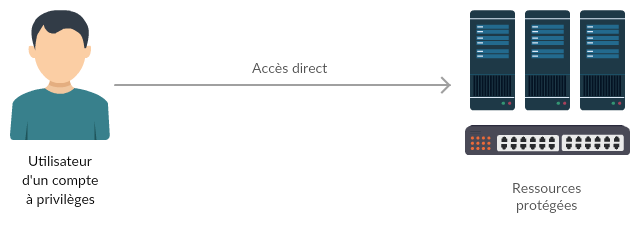
\includegraphics[width=\textwidth]{./images/Schema_ultra_light_sans_PAM.png}
    \caption{Connexion à une ressource protégée sans solution de PAM}
    \label{fig:sans_PAM}
\end{figure}

On remarque qu'ici, les utilisateurs accèdent directement aux ressources protégées avec des mots de passe dédiés à chaque service/application/matériel. Il est donc très fréquent car inévitable que des utilisateurs partagent le même mot de passe. De plus, n'ayant aucune fédération (pas de supervision, ni de traçage), l'utilisateur est apte à effacer ses traces, par exemple en vidant les logs des applications et de ses actions\footnote{Par exemple sous Debian 8, la commande \texttt{cat /dev/null > ~/.bash\_history \&\& history -c \&\& exit} supprime toute action effectuée sur la machine avec le compte courant.}. On ne peut donc pas savoir ce que l'utilisateur a fait, ni quel utilisateur a fait des actions sur la ressource cible.\\
Le diagramme de séquence en \textsc{Figure} \ref{fig:diagseq_sans_PAM} décrit en détail les action qui se déroulent lors d'une telle connexion. Il permet de ausi de mettre en évidence l'absence de contrôle des utilisateurs : aucun registre d'évènements ne prend en compte les actions des utilisateurs. Les utilisaterus se partageant le même mot de passe pour chaque ressource cible, le contrôle n'est ainsi plus mis sur les utilisateurs, mais sur les ressources cibles, ce qui est l'opposé de ce que nous cherchons à faire. La \testsc{Figure} \ref{fig:invcont} schématise cette inversion du contrôle. 

\begin{figure}[!ht]
    \center
    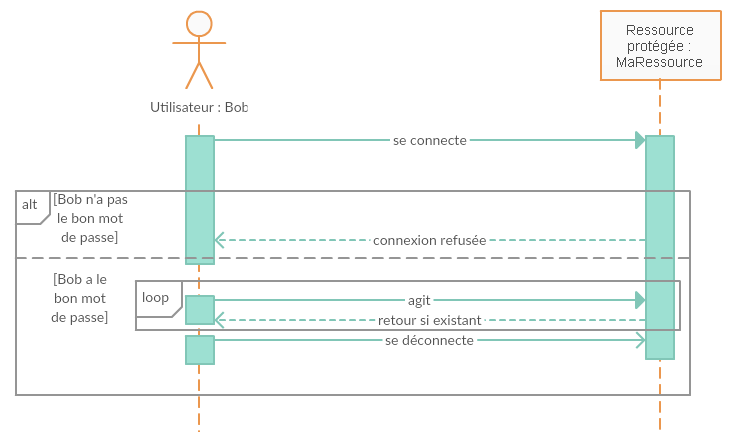
\includegraphics[width=\textwidth]{./images/Sequence_noPAM_use.png}
    \caption{Diagramme de séquence détaillant les actions effectuées lors d'une connexion à une ressource sans solution de PAM}
    \label{fig:diagseq_sans_PAM}
\end{figure}

\begin{figure}[!ht]
    \center
    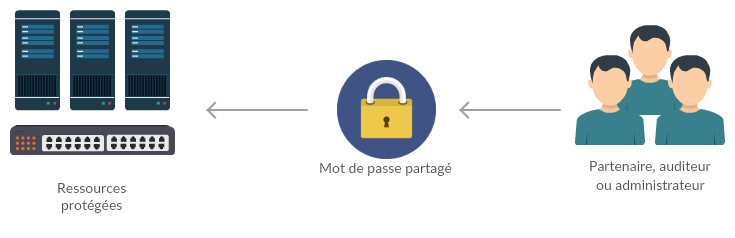
\includegraphics[width=\textwidth]{./images/ressource_centered.png}
    \caption{Schéma mettant en évidence l'inversion du contrôle de sécurité, mis sur les ressources plutôt que sur les utilisateurs}
    \label{fig:invcont}
\end{figure}

\subsubsection{Avec solution de PAM}
\label{par:withpam}

Dans ce scénario, une solution de PAM est en place. Ainsi les utilisateurs n'ont pas d'accès direct aux ressources cible. Toute l'architecture s'articule autour d'un composant central : le contrôleur d'accès appelé \textbf{bastion}. Tout accès à une ressource cible se fait via ce bastion. Cette architecture centralisée est schématisée dans la \textsc{Figure} \ref{fig:schempam}. Nous allons reprendre point par point un scénarion de connexion réussie à une ressource cible (en correspondance avec les étapes de la \textsc{Figure} \ref{fig:schempam}).

\begin{figure}[!ht]
    \center
    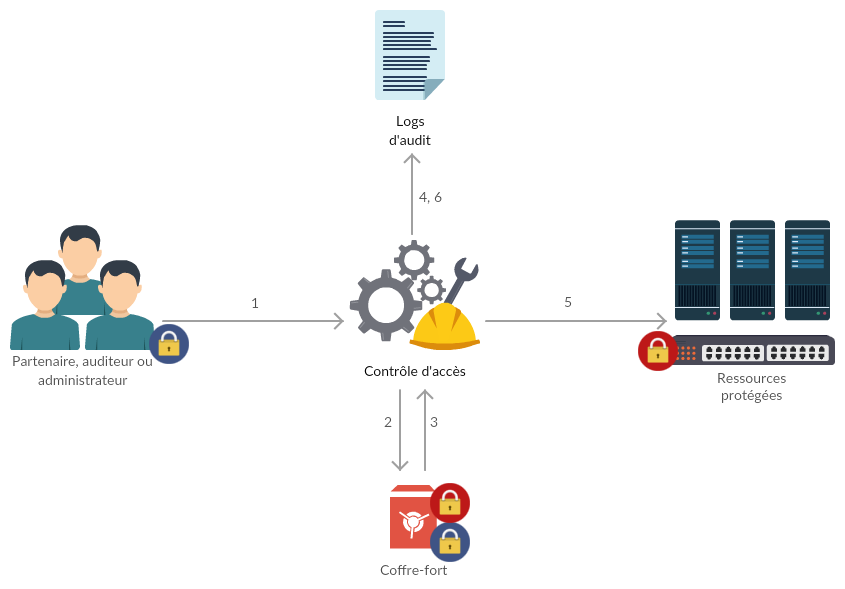
\includegraphics[width=\textwidth]{./images/Schema_PAM.png}
    \caption{Schéma décrivant l'architecture d'une solution de PAM intégrée dans une infrastructure}
    \label{fig:schempam}
\end{figure}

\begin{enumerate}
	\item L'utilisateur se connecte au bastion avec ses crédentiels
\end{enumerate}